\documentclass{scribe}

%====================================================================
%====================================================================
% IMPORTANT: PLEASE UPDATE THE LECTURE INFORMATION BELOW:
\setcounter{lecture}{23} % Lecture number here, from The Big Table on Canvas
\renewcommand{\lectureTitle}{RSA function and RSA encryption}
\renewcommand{\lecturer}{Mahdi Cheraghchi}
\renewcommand{\scribe}{Yi-Wen Tseng}
\renewcommand{\lectureDate}{April 3, 2023} % Date of the lecture
%====================================================================
%====================================================================

\begin{document}

\maketitle

%=============================================================================
%=============================================================================

\section{RSA Function}
In general, public key encryption relies on some computational hardness for security:
\begin{itemize}
    \item \textbf{Diffie-Hellman}: the hardness of discrete log (finding an \textbf{unknown exponent} $a$ given $g^a$) in a group of \textbf{known} order
    \item \textbf{RSA}: the hardness of factoring and finding roots (finding \textbf{unkonwn base} but known exponent) in a group of \textbf{unknown} order
\end{itemize}

\subsection{Mathematical Foundation of RSA Function}
Let $N = p \cdot q$ be the product of two huge distinct primes: $p$ and $q$.
\\
Then, $\mathbf{Z}_N^* = \{a \in \mathbf{Z}_N = \{0, \dots, N-1\}: gcd(a,N) =1\}$
\\
We start with $\mathbf{Z}_N$ and throw out all multiples of $p$ $(0,p,2p, \dots ,(q-1)p)$ and of $q$ $(0,q, \dots, (p-1)q)$ which would double count 0. 
\\
This means $|\mathbf{Z}_N^*| = \varphi(N) = p \cdot q - q -p +1 = (p-1)\cdot (q-1)$.
\\\\
\textbf{Euler's Theorem}: In any group $G$, $\forall  a \in G$, $a^{|G|} = 1 \in G$. 
\\Say $G = \mathbf{Z}_N^*$ $\Rightarrow \forall a \in \mathbf{Z}_N^*$, $a^{\varphi(N)}=a^{(p-1)(q-1)} = 1 (\bmod N)$ 
(Arithmetic  $\bmod N$ is "$ \bmod \varphi(N)$" in the exponent)
\\\\
Take some $e$ such that $gcd(e,\varphi(N)) = 1$ (example: $e$ is a prime such that $e \nmid (p-1)$, $e \nmid (q-1)$ this works)
\\\\
By Euclidean algorithm, we can compute integers $A$ and $B$, which are B\'{e}zout coefficients, such that $Ae+B\varphi(N) = 1$.
\\
\[\Rightarrow A \cdot e = 1 - B \varphi(N) = 1 (\bmod \varphi(N))\]
Define $d = A \bmod \varphi(N)$ is the multiplicative inverse of $e \bmod \varphi(N)$: $d=e^{-1} (\bmod \varphi(N))$ and $d \cdot e = 1 (\bmod \varphi(N))$. (usually choose $e=3$)
\vspace{10mm}

\subsection{RSA Function}
The choice of $N, e, d$ gives us the RSA function and its inverse.
\\\\
\textbf{Definition}: For $N=p \cdot q$ (large distinct primes p, q) and $e \in Z_{\varphi(N)}^*$ with $d = e^{-1} (\bmod \varphi(N))$, the RSA function $RSA _{N,e}: \mathbf{Z}_N^* \rightarrow \mathbf{Z}_N^*$ is a bijection and $RSA _{N,e}(x) = x^e \bmod N $.
\\
The inverse is $RSA _{N,d}(y) = RSA _{N,e}^{-1}(y) = y^d \bmod N$
\\\\
\textbf{Proof}: $RSA_{N,e}$ maps $\mathbf{Z}_N^*$ to $\mathbf{Z}_N^*$ ($\mathbf{Z}_N^*$ is a group with multiplication, which means that the number stays in the group after a series of multiplication with number in the group)
\\
Need to show $RSA _{N,d}= RSA _{N,e}^{-1}$ (inverse function)
\\
Let  $ y  = RSA _{N,e}(x) = x ^e \bmod N$
\[ y ^d = (x^e)^d = x^{ed}  = x^{ed + k \varphi(N)} = x^1 \bmod N = x \bmod N\]
\\\\
RSA function is an example of "trapdoor function." We can efficiently evaluate $RSA_{N,e}$ in the forward direction, and given "trapdoor information" $d$, we can efficiently invert. However, it would be hard to invert without $d$.
\begin{figure}[H]
    \centering
    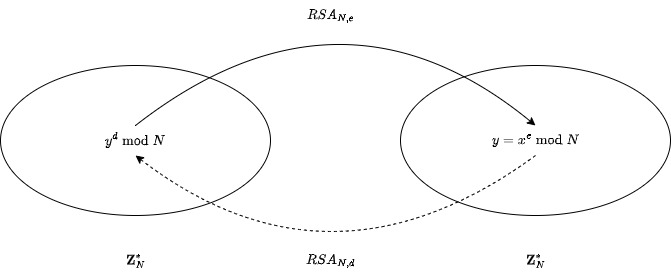
\includegraphics[scale=0.5]{rsa_function.jpg}
    \caption{RSA Function}
\end{figure}
\vspace{10mm}
\section{RSA Encryption}
\subsection{RSA Key Generation}
RSA key generation $GenRSA(1^n)$ works as follows:
\begin{enumerate}
    \item Choose random independent large primes $p,q$ having bit lengths approximately related to n (usually 4096 bits)
    \item Define $N = p \cdot q$. Compute $\varphi(N) = (p-1)(q-1)$
    \item Choose some $e>1$ such that $gcd(e,\varphi(N)) = 1$. Euclid also gives us $d = e^{-1} (\bmod \varphi(N))$
    \item Output $pk = (N,e)$ and $sk = (N,d)$
\end{enumerate}
Common choices for $e$: random, $e=3$ (if $3 \nmid (p-1)$, $3 \nmid (q-1)$), $e = 2^{16} +1 (prime)$. 
\\
We usually choose $e=3, 2^{16} +1$ because there are only two '1' bits in the binary form which makes exponentiation faster.
\vspace{5mm}
\\
\textbf{Definition}: RSA hardness assumption: $\forall \text{ p.p.t } A$
\[Adv^{RSA}(A) = \Pr_{(pk=(N,e), sk) \leftarrow GenRSA(1^n), y \leftarrow \mathbf{Z}_N^*} [A(1^n, (N,e), y) \text{ outputs }x=RSA_{N,e}^{-1}(y)] = negl(n)\]
Given public key $(N,e)$ and a \textbf{RANDOM} $y \in \mathbf{Z}_N^*$, it's hard to find the pre-image $x=y^d = y^{e^{-1}} \bmod N$.
\vspace{5mm}
\\
The definition of advantage is related to the idea of factoring in the way below:
\begin{enumerate}
    \item \textbf{RSA $\le$ Factoring}\\
            RSA is reducible to factoring. If we know how to efficiently factor, we could break RSA.\\
            If there's an efficient algorithm for factoring integers into their prime factors, then there is one for solving RSA.\\
            Given $pk = (N,e)$, $y \in \mathbf{Z}_N^*$. Factor $N=p \cdot q$. Then, $\varphi(N) = (p-1)(q-1)$. $d = e^{-1} \bmod \varphi(N)$ and $y^d \bmod N$ are all easy to compute.
    \item \textbf{Factoring = Finding $\varphi(N)$ from N}\\
            If we know $\varphi(N)$. It could be easy to solve for $p$ and $q$. Because
            \[\varphi(N) = p \cdot q - p - q +1 = (N+1) -p - q \]
            then solve 
            \begin{equation*}
                \begin{cases}
                  p+q = (N+1) - \varphi(N)\\
                  p \cdot q = N
                \end{cases}\,
            \end{equation*}
    \item \textbf{Factoring = Finding $d$ from $(N,e)$}\\
            We know $e \cdot d - 1 = k \cdot \varphi(N)$ for some k.\\
            Through some computation, it is enough to have a multiple of $\varphi(N)$ ($k \cdot \varphi(N)$) to recover a factoring of $N$.
\end{enumerate}
\textbf{*Notice}: We do not know whether factoring is reducible to RSA. Factoring is the best-known attack against RSA, and factoring is thought to be hard. If there is any other way to find $p$ and $q$, breaking RSA could be easy.
\vspace{5mm}
\subsection{RSA Encryption and Decryption}
\subsubsection{"Textbook RSA" Encryption (DO NOT USE!!! It is insecure.)}
\begin{equation*}
    \begin{cases}
      Enc(pk = (N, e), m \in \mathbf{Z}_N^*): \text{ output } c= RSA_{N,e}(m) = m^e \bmod N \\
      Dec(sk = (N, d), c \in \mathbf{Z}_N^*): \text{ output } m = RSA_{N,d}(c) = c^d \bmod N
    \end{cases}\,
\end{equation*}
It meets the correctness requirement. However, it is not CPA-secure because the encryption is deterministic.

%=============================================================================

\subsubsection{Better Approach}
Apply $RSA_{N,e}$ on a random $x \leftarrow \mathbf{Z}_N^*$. Then, we know $x$ is hard to recover from $y=RSA_{N,e}(x)$.
\\
We first use a hash function on $x$ and encrypt message $m$:
\[c = (y=RSA_{N,e}(x) = x^e \bmod N, H(x) \oplus m)\]  

\section{Additional Note about RSA}
* RSA is used in limited security, and we can think of it as bootstrapping a symmetric protocol.
\\
* x needs to be large to make $x^e$ wrap around $N$. Otherwise, it could be easy to recover x.
%=============================================================================
%=============================================================================

\bibliographystyle{alpha}
% Uncomment below if you have any references:
%\bibliography{\jobname}

%=============================================================================
%=============================================================================

\end{document}
